\documentclass{beamer}
\usepackage{beamerthemesplit}
\usepackage{wrapfig}
\usepackage{verbatim}
\usetheme{SPbGU}
\usepackage{pdfpages}
\usepackage{amsmath}
\usepackage{cmap} 
\usepackage[T2A]{fontenc} 
\usepackage[utf8]{inputenc}
\usepackage[english,russian]{babel}
\usepackage{indentfirst}
\usepackage{amsmath}
\usepackage{tikz}
\usepackage{multirow}
\usepackage[noend]{algpseudocode}
\usepackage{algorithm}
\usepackage{algorithmicx}
\usetikzlibrary{shapes,arrows}
\usepackage{fancyvrb}
\usepackage{tikz}
\usepackage{pgfplots}
\usepackage{sidecap}
\pgfplotsset{compat=1.9}
\newtheorem{rutheorem}{Теорема}
\newtheorem{ruproof}{Доказательство}
\newtheorem{rudefinition}{Определение}
\newtheorem{rulemma}{Лемма}
\beamertemplatenavigationsymbolsempty

\title[]{Зачем биологам синтаксический анализ}
% То, что в квадратных скобках, отображается в левом нижнем углу. 
\institute[СПбГУ]{
    Санкт-Петербургский государственный университет \\
    Лаборатория языковых инструментов JetBrains}

% То, что в квадратных скобках, отображается в левом нижнем углу.
\author[Артём Горохов]{Артём Горохов}
\date{15 октября 2016г.}

\begin{document}
    
\definecolor{red}{RGB}{255,0,0}

\begin{frame}
    \begin{center}
        {\includegraphics[width=1.5cm]{pictures/SPbGU_Logo.png}}
    \end{center}
    \titlepage
\end{frame}

\begin{frame}
   	\frametitle{Биоинформатика}
   	\begin{itemize}
        \item Множество задач, связанных с обработкой и пониманием биологических данных
   		\item Одна из задач --- поиск организмов в метагеномных сборках
   	\end{itemize}
\end{frame}

\begin{frame}
    \frametitle{Геном}
    \begin{itemize}
        \item Геном --- длинная последовательность нуклеотидов
        \item На деле строка над алфавитом \{A, C, G, U\}
    \end{itemize}
\end{frame}

\begin{frame}
    \frametitle{Получение данных}
    \begin{tabular}{p{5cm} p{7cm}}
        \begin{itemize}
            \item Из биологического материала получаются последовательности строчек длиной около 100 символов
            \item Эти кусочки склеиваются в более длинные строки
            \item Множество строчек --- сборка
            \item Данных очень много, так что строится граф, задающий множество полученных строк
        \end{itemize}
        &
        \begin{figure}[b]
            \centering
            \includegraphics[width=6.5cm]{pictures/readsAssembly.png}  
        \end{figure}
    \end{tabular}
\end{frame}

\begin{frame}
    \frametitle{Сборки}
    В зависимости от биологического материала, из которого получаются данные, сборки
    бывают:
    \begin{itemize}
        \item single-cell, multi-cell: клетки одного штамма
        \item \textbf{метагеномные}: данные взяты из среды обитания целевой колонии, в которой были как её представители, так и соседствующих
    \end{itemize}
\end{frame}

\begin{frame}
    \frametitle{Что ищем}
    \begin{tabular}{p{6cm} p{5cm}}
        \begin{itemize}
            \item Хочется понять что у нас в сборке
            \item Такие последовательности как тРНК, рРНК хорошо характеризуют организм которому они принадлежат
            \item У этих последовательностей есть вторичная структура, которая может быть описана КС-грамматикой
        \end{itemize}
        &
        \begin{figure}[b]
            \centering
            \multirow{-3}*{\includegraphics[width=5.2cm]{pictures/TRNA.png}}
            %\caption{Вторичная структура тРНК}
        \end{figure}
        \\
        $$
        GGAAGAUCG...GCA...  =>
        $$
        &
    \end{tabular}  
\end{frame}

\begin{frame}
    \frametitle{Грамматика для кусочка тРНК}
        \begin{tabular}{p{6cm} p{5cm}}
            {$\begin{aligned}
                START\ =&\ STEM \\
                STEM\ =&\ a\ STEM\ u \\
                      |&\ u\ STEM\ a \\
                      |&\ c\ STEM\ g \\
                      |&\ g\ STEM\ c \\
                      |&\ g\ STEM\ u \\
                      |&\ u\ STEM\ g \\
                      |&\ ANY^{*}[4..7] \\
                ANY\ =&\ a\ |\ u\ |\ g\ |\ c \\
                \end{aligned}$}
            &
            \multirow{-7}*{\includegraphics[width=3cm]{pictures/TRNAPart.png}}
        \end{tabular}
\end{frame}

\begin{frame}
    %\frametitle{Вторичная структура 16s}
    \begin{tabular}{p{4cm} p{7cm}}
        Вторичная структура 16s рРНК
        &
        \multirow{-7}*{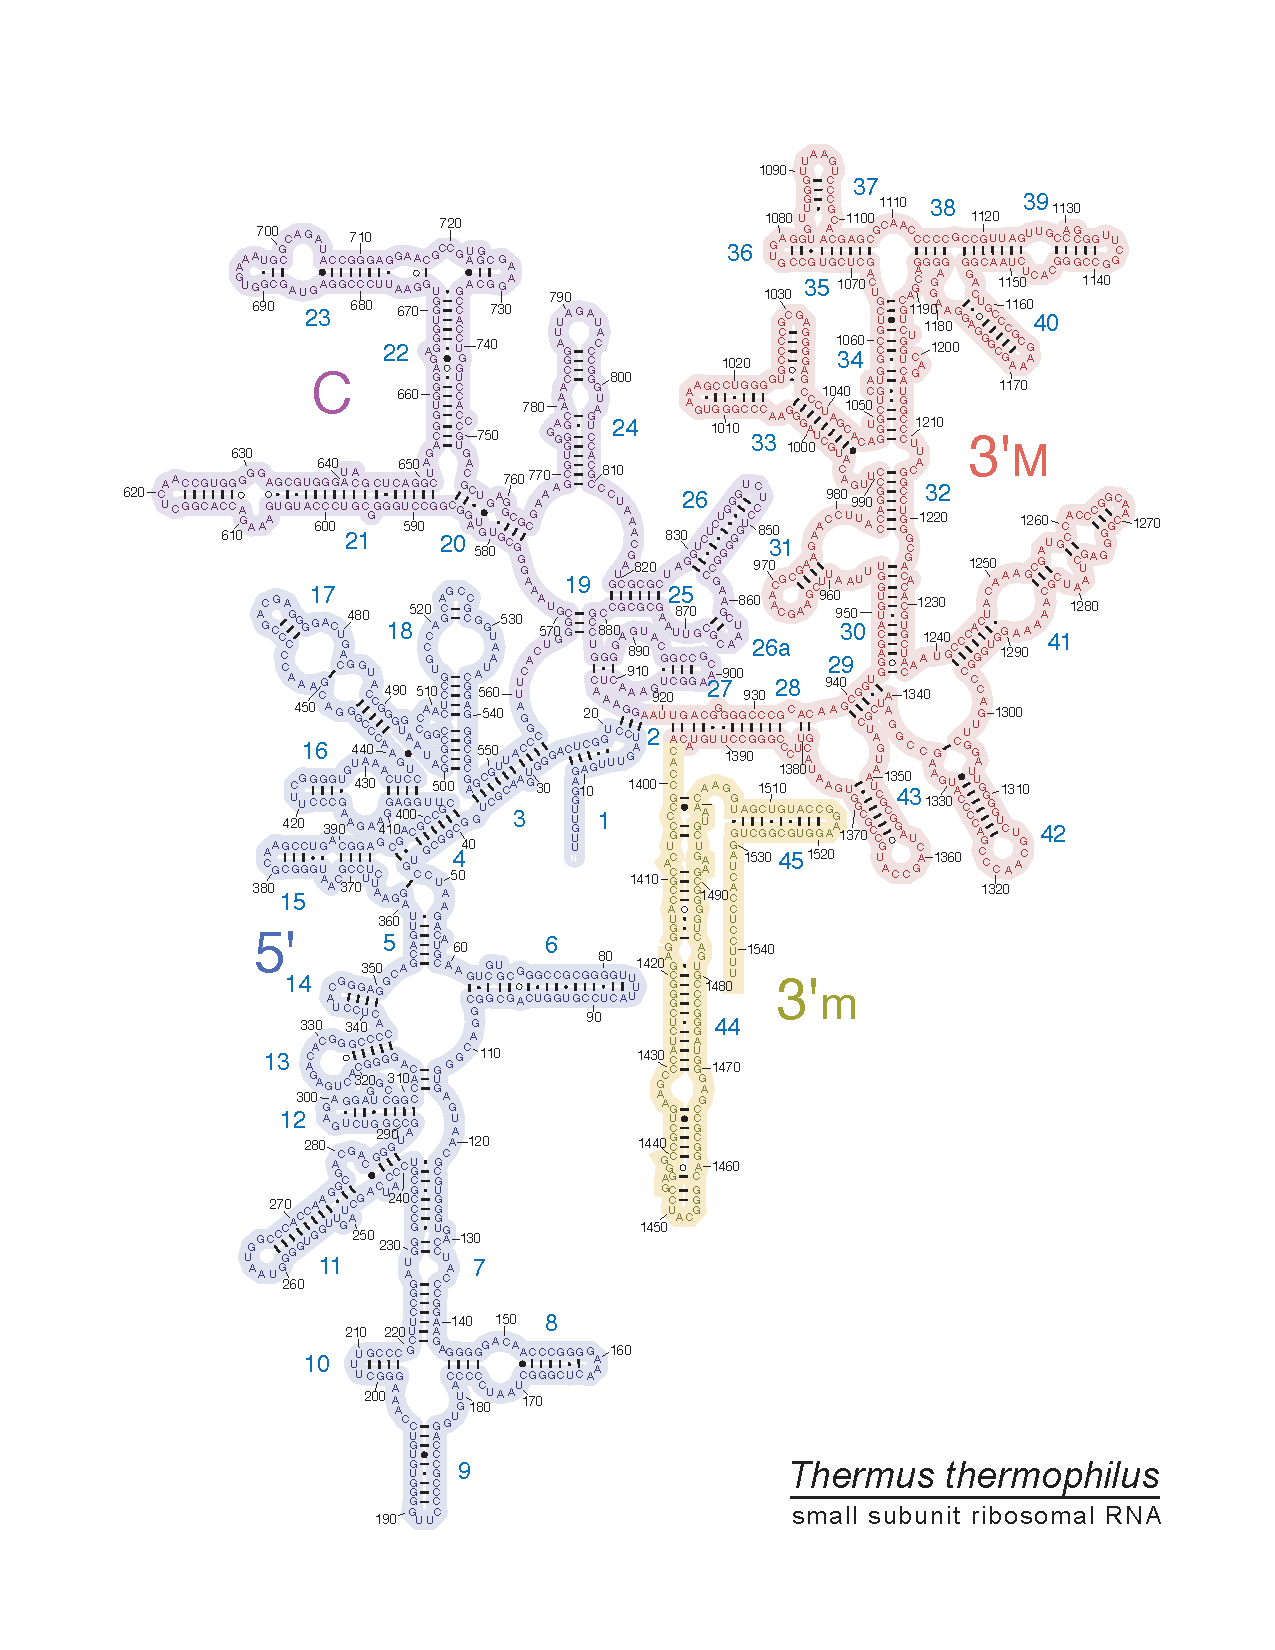
\includegraphics[width=6.5cm]{pictures/thermus_16s_2ndry.pdf}}
    \end{tabular}
\end{frame}

\begin{frame}
    \frametitle{Цель и задачи}
    \textbf{Целью} работы является с помощью синтаксического анализа находить в метагеномной сборке структуры, принадлежащие организмам
    
    \textbf{Задачи}:
    \begin{itemize}
        \item Адаптировать существующий алгоритм под специфику задачи
        \item Провести экспериментальные исследования работы алгоритма
    \end{itemize}
\end{frame}

\begin{frame}
    \frametitle{Graph parsing}
    \begin{itemize}
        \item В лаборатории созданы алгоритмы
        \item Реализован инструмент, основанный на алгоритме GLL
        \item Умеет решать задачу поиска линейных цепочек в графе, удовлетворяющих КС-грамматике
    \end{itemize}
\end{frame}

\begin{frame}
	\frametitle{GLL}
	\begin{itemize}
		\item Разбор осуществляется при помощи дескрипторов
        \item Дескриптор --- четвёрка (слот, позиция во входе, дерево, вершина стека)
		\item На каждом шаге достаём дескриптор из очереди и разобрав очередной символ создаём новые дескрипторы
	\end{itemize}
\end{frame}

\begin{comment}
\begin{frame}
	\frametitle{GLL}
	\begin{figure}[t]
		\begin{tabular}{p{3cm} p{3cm} p{3cm}}
			Вход: a a b
			&
			\multirow{1}*{\includegraphics[width=3cm]{pictures/GLLtree0.pdf}}
			&
			\multirow{1}*{\includegraphics[width=3cm]{pictures/GLLtree1.pdf}}
			\\ & & \\
			Грамматика:& & \\
			{$\begin{aligned}
				S\ =&\ A\ B \\
				A\ =&\ a\ a \\
				|&\ a \\
				B\ =&\ b \\
				|&\ a\ b
				\end{aligned}$} & &
		\end{tabular}
		
	\end{figure}
\end{frame}

\begin{frame}
	\frametitle{GLL для графов}
	\begin{tabular}{p{7cm} p{5cm}}
		\begin{itemize}
			\item На вход поступает граф, задающий все входные цепочки
			\item На рёбрах терминалы
		\end{itemize}
		&
		% Картинка
		\multirow{-4}*{\includegraphics[width=3cm]{pictures/graphGLLexample.pdf}}
		\\ &
		\\ &
		\\ 
		$$
		\{A B C D;
		A M C D;
		A E K D \} =>
		$$ &
	\end{tabular}
\end{frame}
\end{comment}

\begin{frame}
    \frametitle{Особенности графа}
    \begin{itemize}
        \item Полученные метагеномные сборки не поддаются анализу без предварительных преобразований
        \item Infernal позволяет распознавать структуры в линейном входе
        \item Рёбра, длиннее искомых структур можно делить на части и проверять с помощью Infernal
        \item После фильтрации рёбер граф распадается на компоненты связности, на которых алгоритм можно запускать анализатор независимо
    \end{itemize}
\end{frame}

\begin{frame}
    \frametitle{Отказ от построения дерева}
    \begin{itemize}
        \item Синтаксический анализатор возвращает лишь границы и длину найденных цепочек
        \item Восстановление цепочки идёт путём извлечения подграфа, состоящего из путей заданной длины
        \item Ложные фильтруются с помощью Infernal
    \end{itemize}
    
    \begin{figure}[b]
        \centering
        \includegraphics[width=8cm]{pictures/noTree.pdf}  
    \end{figure}
\end{frame}

\begin{frame}
    \frametitle{Преобразование грамматики}
    \begin{itemize}
        \item Грамматика для 16s сильно неоднозначная и довольно большая 
        \item Из-за этого количество слотов в грамматике избыточно
        \item В процессе разбора создаётся большое количество ненужных дескрипторов 
    \end{itemize} 
\end{frame}


\begin{frame}
    \frametitle{Преобразование грамматики к автомату}
    \begin{tabular}{p{5cm} p{4cm}}
        Грамматика & Автомат \\
          &   \\
          &   \\
        {$\begin{aligned}
            START\ =&\ STEM \\
            STEM\ =&\ a\ STEM\ u \\
            |&\ u\ STEM\ a \\
            |&\ c\ STEM\ g \\
            |&\ g\ STEM\ c \\
            |&\ g\ STEM\ u \\
            |&\ u\ STEM\ g \\
            |&\ ANY^{*}[3..6] \\
            ANY\ =&\ a\ |\ u\ |\ g\ |\ c \\
            \end{aligned}$}
        &
        \multirow{-8}*{\includegraphics[height=7cm]{pictures/initialNFA.pdf}}
    \end{tabular}
\end{frame}

\begin{frame}
    \frametitle{Минимизация автомата}
    \begin{tabular}{p{6cm} p{5.5cm}}
        Изначальный автомат & Минимизированый автомат \\
        &   \\
        &   \\
        &   \\
        &   \\
        &   \\
        &   \\
        &   \\
        &   \\
        &   \\
        &   \\
        &   \\
        &   \\
        \multirow{-13}*{\includegraphics[height=7cm]{pictures/initialNFA.pdf}}
        &
        \multirow{-13}*{\includegraphics[height=7cm]{pictures/minimizedDFA.pdf}}
    \end{tabular}
\end{frame}

\begin{frame}
    \frametitle{Эксперименты}
    Результаты работы на сборке, состоящей из 59000 вершин и 87000 рёбер
    \begin{center}
        \begin{tabular}{ p{2.5cm} | p{2cm} | p{2.5cm}}
                                        & начальная грамматика & мин. автомат \\ \hline
            Время работы                & 10 ч.                & 3 ч. 40 мин. \\ \hline
            Кол-во слотов /состояний    & 41                   & 17           \\ \hline
        \end{tabular}
    \end{center}
    Эксперименты проводились на машине с 32 ГБ RAM и CPU core i7-4790
    
\end{frame}

\begin{frame}
    \frametitle{Результаты}
    \begin{itemize}
        \item Разработан механизм подготовки сборок к синтаксическому анализу
        \item GLL адаптирован под распознавание по грамматике в форме EBNF
        \item Проведены эксперименты на части грамматики 16s РНК
    \end{itemize}
\end{frame}

\begin{frame}
    \frametitle{Направление работ}
    \begin{itemize}
        \item Детальный анализ качества результата
        \item Возможно, можно сильнее фильтровать граф, например применяя infernal 
        \item Поиск полноразмерных 16s
    \end{itemize}
\end{frame}


\end{document}
